\documentclass[12pt,a4paper,titlepage,oneside]{article}
\usepackage{report}
\usepackage{url}
\usepackage{amsmath}

\title{Assignment 1}

\author{Vorname1 Nachname1, \matrnr 0000000   \\
         {\small e00000000@vmars.tuwien.ac.at} \\
        Vorname2 Nachname2, \matrnr 99012345 \\
         {\small e99012345@student.tuwien.ac.at}
}
\begin{document}

% create titlepage
\maketitle

%\tableofcontents
%\newpage

%------------------------------------------------------------------
\section{Problem 1}

\subsection{Problem Statement}
\label{problem:1}

In directory \texttt{insertion\_sort}, implement the function
\texttt{main.c:run()}. This routine should call the insertion
sort routine several times, with different arrays of size $32$.

\begin{itemize}
\item[Q1:] What is the minimum and maximum number of times the statement
           labeled \texttt{insertion\_sort\_move} might be
           executed for some input data (assuming an array size of $N$)?
\item[Q2:] How many test runs do you need to cover all possible paths through
           the function?
\item[Q3:] Report the minimum and maximum execution times measured for
           your test runs of insertion sort.
\end{itemize}


\subsection{Solution}
% TODO

\subsection{Listings}
% TODO

%------------------------------------------------------------------
\newpage
\section{Problem 2}

\subsection{Problem Statement}
\label{problem:2}

Add loop bounds and additional flow facts for
\texttt{insertion\_sort.c:insertion\_sort()}, and analyze the WCET of
\texttt{insertion\_sort}.

\begin{itemize}

\item[Q1:]
  What is the WCET of insertion\_sort, assuming the array has 8,16,32 or 64
  elements? Compare the WCET for arrays of size $32$ with your measurement
  results.

\item[Q2:]
  What other properties of the input (despite the size of the array) have a
  significant impact on the execution time? How could you take them into
  account during static WCET analysis?

\item[Q3:]
  Now try compiling with \texttt{-O1} (cf.\ the Makefile).  Try to add your
  flow facts for array size $32$.  This might require a different method than
  source code annotations.  List the maximally observed execution time and the
  WCET from analysis, and compare them to the results obtained with
  \texttt{-O0}.

\item[Q4:] (Bonus)
  Figure~\ref{fig:cfg.insertion_sort} depicts the \emph{control-flow graph}
  (CFG) of the \texttt{insertion\_sort} function as exported from the compiler
  intermediate representation.
  %
  Formulate an ILP problem to calculate the WCET.  That is, specify a set of
  (integer) variables, a linear objective function, and a set of linear
  constraints, such that the solution to the problem is an upper bound for the
  execution time of the program.  The linear constraints consist of the
  structural constraints given by the CFG and the flow constraints you
  specified.
  For the basic block costs, assume a very simple model and use the costs
  given in Table~\ref{tab:cfg.insertion_sort}.
  Write an input file for an ILP solver%
  \footnote{Recommendation: \url{http://sourceforge.net/projects/lpsolve}},
  and check the solution calculated by the solver.
  Do not forget to give the number of times each basic block is executed in
  your solution.

\end{itemize}


\begin{figure}
  \centering
  \begin{minipage}[c]{.6\linewidth}
    %\vspace{0pt}
    \centering
    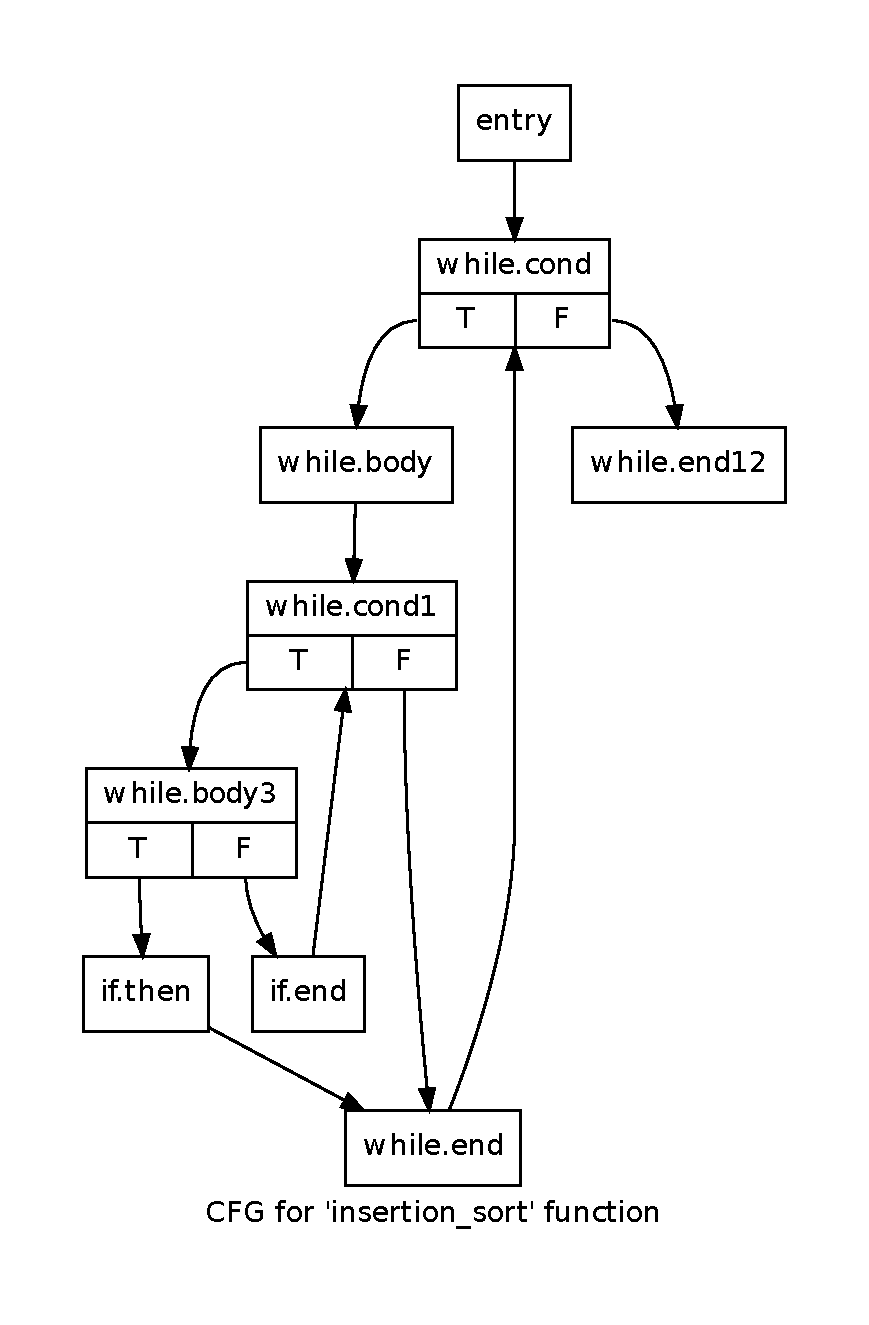
\includegraphics[width=0.90\linewidth]{../assignment/cfg_insertion_sort}
  \end{minipage}%
  \begin{minipage}[c]{.3\linewidth}
    %\vspace{0pt}
    \centering
    \small
    \begin{tabular}{|l|r|}
      \hline
      Basic Block & Cost \\
      \hline
      entry & 12 \\
      while.cond & 6 \\
      while.body & 15 \\
      while.cond1 & 4 \\
      while.body3 & 11 \\
      if.then & 1 \\
      if.end & 21 \\
      while.end & 16 \\
      while.end12 & 1 \\
      \hline
    \end{tabular}
  \end{minipage}
  \caption{Control-Flow Graph for \texttt{insertion\_sort} (from LLVM IR)
           and costs for the execution of basic blocks.}
  \label{fig:cfg.insertion_sort}
\end{figure}

\clearpage


\subsection{Solution}
% TODO

\subsection{Listings}
% TODO

%------------------------------------------------------------------
\newpage
\section{Problem 3}

\subsection{Problem Statement}
\label{problem:3}

First, focus on the analysis of \texttt{task.c:merge\_samples()}.  The loop
bounds in this function depend on the input-data dependent parameter
\texttt{@inputcount}, defined to be the maximal value of
\texttt{input->input\_count}. Add loop bounds and flow facts for
\texttt{merge\_samples}, and analyze its WCET assuming that
$\texttt{@inputcount} \leq 64$.

\begin{itemize}

\item[Q1:]
  Describe and justify the loop bounds and flow facts used in the WCET analysis
  of \texttt{merge\_samples}.

\item[Q2:]
  What is the maximum execution time observed for this function? What is the
  analyzed WCET? In case they do not coincide, discuss reasons for the
  impreciseness in the static analysis.

\item[Hint:]
  For measurements, you might want to rely on or start with the test bench
  implemented in\\
  \texttt{main.c:test\_merge\_samples()}.

\item[Hint:]
  Division is implemented in software for the Patmos architecture. We replaced
  the division in the interpolation routine by a lookup table for small values,
  to simplify the analysis problem. You do not need to worry about the analysis
  of \texttt{iinterpolate16}; simply use the following annotations:

\end{itemize}

\begin{verbatim}
  include "llvm.ais";
  instruction "iinterpolate16" + 1 calls is never executed;
  instruction "iinterpolate16" + 2 calls is never executed;
\end{verbatim}


\subsection{Solution}
% TODO

\subsection{Listings}
% TODO

%------------------------------------------------------------------
\newpage
\section{Problem 4}

\subsection{Problem Statement}
\label{problem:4}

Next, analyze the \texttt{fft()} function called in \texttt{task.c}. Try to
find loop bounds for the Fast Fourier Transform implementation
(\texttt{fixedpoint.c:fp\_radix2fft\_withscaling()}) first, and add a flow
constraint relating the execution frequency of the inner loop's body with
the function's execution frequency.

\begin{itemize}

\item[Q1:]
  Describe and justify the flow facts found for
  \texttt{fp\_radix2fft\_withscaling}, and \texttt{fft}.

\item[Q2:]
  What is the maximum execution time observed for this function? What
  is the analyzed WCET?

\item[Q3:]
  For the FFT implementation \texttt{fp\_radix2fft\_withscaling}, is it safe to
  use the loop iteration counts observed during a test run? Justify your
  answer.

\item[Hint:]
  For measurements, you might want to rely on or start with the test
  implementation \texttt{main.c:test\_fft()}

\end{itemize}


\subsection{Solution}
% TODO

\subsection{Listings}
% TODO

%------------------------------------------------------------------
\newpage
\section{Problem 5}

\subsection{Problem Statement}
\label{problem:5}
The final goal is to analyze the WCET of \texttt{task.c:task()}.

\begin{itemize}

\item[Q1:]
  First, calculate the WCET of \texttt{check\_sin} and \texttt{check\_square}.
  Then, try to give a rough estimate on the WCET by combining the WCET's of
  \texttt{merge\_samples}, \texttt{fft}, \texttt{check\_sin} and
  \texttt{check\_square}. Clearly state how you combined the WCETs, and compare
  the resulting value with the maximum observed execution time of these
  functions, combined in the same way.

\item[Q2:]
  Add a flow fact for the indirect call in \texttt{task}, calculate the WCET of
  \texttt{task}, and compare it to the maximum execution time observed.

\end{itemize}


\subsection{Solution}
% TODO

\subsection{Listings}
% TODO

%------------------------------------------------------------------
\newpage
\section{Reflections}

%\subsection{Problem Statement}
\label{problem:6}

Answer the following questions:

\begin{itemize}

\item[Q1:]
  How much time did you spend writing annotations and analyzing the code?
  Was it less or more than you expected?

\item[Q2:]
  What problems did you encounter during this assignment?

\item[Q3:]
  As you learned, sometimes it is necessary to annotate the assembly code.
  Why? What problems can you see because of this?

\end{itemize}


\subsection{Answers}
% TODO


\end{document}

